\let\negmedspace\undefined
\let\negthickspace\undefined
\documentclass[journal]{IEEEtran}
\usepackage[a5paper, margin=10mm, onecolumn]{geometry}
\usepackage{lmodern}
\usepackage{tfrupee}
\setlength{\headheight}{1cm}
\setlength{\headsep}{0mm}
\usepackage{gvv-book}
\usepackage{gvv}
\usepackage{cite}
\usepackage{amsmath,amssymb,amsfonts,amsthm}
\usepackage{algorithmic}
\usepackage{graphicx}
\usepackage{textcomp}
\usepackage{xcolor}
\usepackage{txfonts}
\usepackage{listings}
\usepackage{enumitem}
\usepackage{mathtools}
\usepackage{gensymb}
\usepackage{comment}
\usepackage[breaklinks=true]{hyperref}
\usepackage{tikz}
\usepackage{tkz-euclide}
\usepackage{listings}
\def\inputGnumericTable{}
\usepackage[latin1]{inputenc}
\usepackage{color}
\usepackage{array}
\usepackage{longtable}
\usepackage{calc}
\usepackage{multirow}
\usepackage{hhline}
\usepackage{ifthen}
\usepackage{lscape}
\usetikzlibrary{matrix}

\begin{document}

\bibliographystyle{IEEEtran}
\vspace{3cm}

\title{10.4.ex.2}
\author{EE24BTECH11011-PRANAY}
{\let\newpage\relax\maketitle}

\renewcommand{\thefigure}{\theenumi}
\renewcommand{\thetable}{\theenumi}
\setlength{\intextsep}{10pt}

\numberwithin{equation}{enumi}
\numberwithin{figure}{enumi}
\renewcommand{\thetable}{\theenumi}

\textbf{Question:}

Find the roots of the quadratic equation:
\begin{align}
    (x-2)^2 + 1 = 2x - 3
\end{align}

\solution

Rearranging terms,
\begin{align}
    (x-2)^2 + 1 - (2x - 3) &= 0 \\
    x^2 - 4x + 4 + 1 - 2x + 3 &= 0 \\
    x^2 - 6x + 8 &= 0
\end{align}

\textbf{Theoretical solution (Quadratic formula):}

The roots are given by:
\begin{align}
    x &= \frac{-b \pm \sqrt{b^2 - 4ac}}{2a} \\
    x &= \frac{6 \pm \sqrt{36 - 32}}{2} \\
    x &= \frac{6 \pm 2}{2} \\
    x &= 4 \text{ and } x = 2
\end{align}

\textbf{Computational solution:}

(1) \textbf{Eigenvalues of Companion Matrix:}

The roots of a polynomial equation $x^n + b_{n-1}x^{n-1} + \dots + b_1x + b_0 = 0$ can be found by computing the eigenvalues of the companion matrix \brak{C}.
\begin{align}
    C = \myvec{0 & 1 \\ -b_0 & -b_1}
\end{align}

For the equation $x^2 - 6x + 8 = 0$, we have:
\begin{align}
    b_0 = 8, \quad b_1 = -6
\end{align}
\begin{align}
    C = \myvec{0 & 1 \\ -8 & 6}
\end{align}

Using eigenvalue decomposition, the roots are:
\begin{align}
    x_1 = 4, \quad x_2 = 2
\end{align}

(2) \textbf{Newton-Raphson iterative method:}

The function and its derivative are:
\begin{align}
    f(x) &= x^2 - 6x + 8 \\
    f'(x) &= 2x - 6
\end{align}

Difference equation:
\begin{align}
    x_{n+1} &= x_n - \frac{f(x_n)}{f'(x_n)} \\
    x_{n+1} &= x_n - \frac{x_n^2 - 6x_n + 8}{2x_n - 6}
\end{align}

Starting with initial guesses:
\begin{align}
    x_0 &= 3 \text{ converges to } 2 \\
    x_0 &= 5 \text{ converges to } 4
\end{align}

\textbf{Verification:}

Substituting $x = 4$:
\begin{align}
    (4-2)^2 + 1 &= 2(4) - 3 \\
    4 + 1 &= 8 - 3 \\
    5 &= 5
\end{align}

Substituting $x = 2$:
\begin{align}
    (2-2)^2 + 1 &= 2(2) - 3 \\
    0 + 1 &= 4 - 3 \\
    1 &= 1
\end{align}

Hence, the roots are verified.

\begin{figure}[h]
\centering
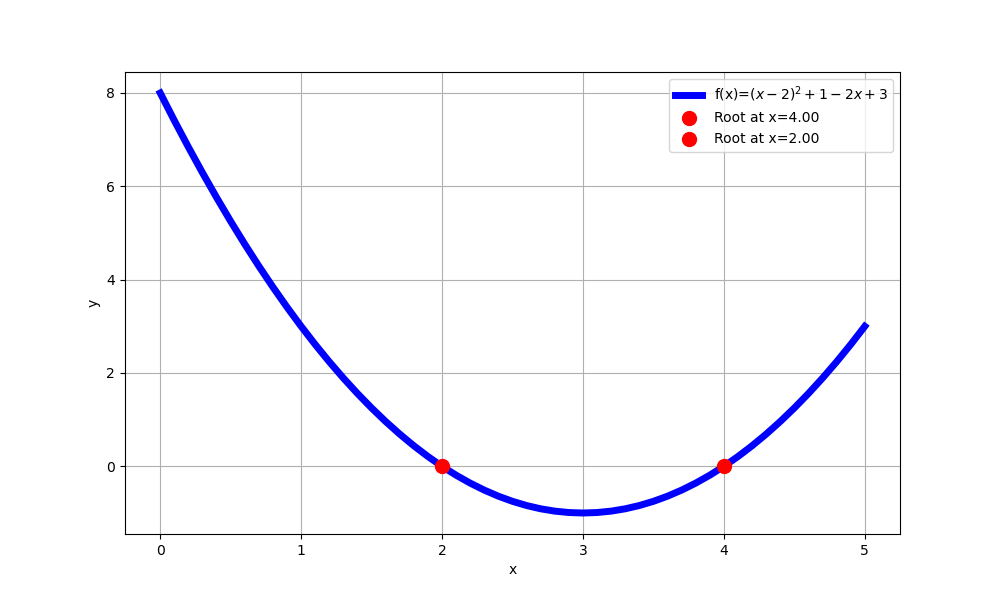
\includegraphics[width=\columnwidth]{figs/fig.png}
\caption{Plot using Newton-Raphson method}
\label{fig:Plot1} 
\end{figure}
\end{document}
\end{document}

